%% BioMed_Central_Tex_Template_v1.05
%%                                      %
%  bmc_article.tex            ver: 1.05 %
%                                       %


%%%%%%%%%%%%%%%%%%%%%%%%%%%%%%%%%%%%%%%%%
%%                                     %%
%%  LaTeX template for BioMed Central  %%
%%     journal article submissions     %%
%%                                     %%
%%         <27 January 2006>           %%
%%                                     %%
%%                                     %%
%% Uses:                               %%
%% cite.sty, url.sty, bmc_article.cls  %%
%% ifthen.sty. multicol.sty		       %%
%%									   %%
%%                                     %%
%%%%%%%%%%%%%%%%%%%%%%%%%%%%%%%%%%%%%%%%%


%%%%%%%%%%%%%%%%%%%%%%%%%%%%%%%%%%%%%%%%%%%%%%%%%%%%%%%%%%%%%%%%%%%%%
%%                                                                 %%	
%% For instructions on how to fill out this Tex template           %%
%% document please refer to Readme.pdf and the instructions for    %%
%% authors page on the biomed central website                      %%
%% http://www.biomedcentral.com/info/authors/                      %%
%%                                                                 %%
%% Please do not use \input{...} to include other tex files.       %%
%% Submit your LaTeX manuscript as one .tex document.              %%
%%                                                                 %%
%% All additional figures and files should be attached             %%
%% separately and not embedded in the \TeX\ document itself.       %%
%%                                                                 %%
%% BioMed Central currently use the MikTex distribution of         %%
%% TeX for Windows) of TeX and LaTeX.  This is available from      %%
%% http://www.miktex.org                                           %%
%%                                                                 %%
%%%%%%%%%%%%%%%%%%%%%%%%%%%%%%%%%%%%%%%%%%%%%%%%%%%%%%%%%%%%%%%%%%%%%


\NeedsTeXFormat{LaTeX2e}[1995/12/01]
\documentclass[10pt]{bmc_article}    



% Load packages
\usepackage{cite} % Make references as [1-4], not [1,2,3,4]
\usepackage{url}  % Formatting web addresses  
\usepackage{ifthen}  % Conditional 
\usepackage{multicol}   %Columns
\usepackage[utf8]{inputenc} %unicode support
%\usepackage[applemac]{inputenc} %applemac support if unicode package fails
%\usepackage[latin1]{inputenc} %UNIX support if unicode package fails
\urlstyle{rm}
 
 
%%%%%%%%%%%%%%%%%%%%%%%%%%%%%%%%%%%%%%%%%%%%%%%%%	
%%                                             %%
%%  If you wish to display your graphics for   %%
%%  your own use using includegraphic or       %%
%%  includegraphics, then comment out the      %%
%%  following two lines of code.               %%   
%%  NB: These line *must* be included when     %%
%%  submitting to BMC.                         %% 
%%  All figure files must be submitted as      %%
%%  separate graphics through the BMC          %%
%%  submission process, not included in the    %% 
%%  submitted article.                         %% 
%%                                             %%
%%%%%%%%%%%%%%%%%%%%%%%%%%%%%%%%%%%%%%%%%%%%%%%%%                     


%\def\includegraphic{}
%\def\includegraphics{}
\usepackage{graphicx}



\setlength{\topmargin}{0.0cm}
\setlength{\textheight}{21.5cm}
\setlength{\oddsidemargin}{0cm} 
\setlength{\textwidth}{16.5cm}
\setlength{\columnsep}{0.6cm}

\newboolean{publ}

%%%%%%%%%%%%%%%%%%%%%%%%%%%%%%%%%%%%%%%%%%%%%%%%%%
%%                                              %%
%% You may change the following style settings  %%
%% Should you wish to format your article       %%
%% in a publication style for printing out and  %%
%% sharing with colleagues, but ensure that     %%
%% before submitting to BMC that the style is   %%
%% returned to the Review style setting.        %%
%%                                              %%
%%%%%%%%%%%%%%%%%%%%%%%%%%%%%%%%%%%%%%%%%%%%%%%%%%
 

%Review style settings
%\newenvironment{bmcformat}{\begin{raggedright}\baselineskip20pt\sloppy\setboolean{publ}{false}}{\end{raggedright}\baselineskip20pt\sloppy}

%Publication style settings
\newenvironment{bmcformat}{\fussy\setboolean{publ}{true}}{\fussy}



% Begin ...
\begin{document}
\begin{bmcformat}


%%%%%%%%%%%%%%%%%%%%%%%%%%%%%%%%%%%%%%%%%%%%%%
%%                                          %%
%% Enter the title of your article here     %%
%%                                          %%
%%%%%%%%%%%%%%%%%%%%%%%%%%%%%%%%%%%%%%%%%%%%%%

\title{Applications of InChI in cheminformatics with the CDK and Bioclipse}
 
%%%%%%%%%%%%%%%%%%%%%%%%%%%%%%%%%%%%%%%%%%%%%%
%%                                          %%
%% Enter the authors here                   %%
%%                                          %%
%% Ensure \and is entered between all but   %%
%% the last two authors. This will be       %%
%% replaced by a comma in the final article %%
%%                                          %%
%% Ensure there are no trailing spaces at   %% 
%% the ends of the lines                    %%     	
%%                                          %%
%%%%%%%%%%%%%%%%%%%%%%%%%%%%%%%%%%%%%%%%%%%%%%



\author{Ola Spjuth\correspondingauthor$^{1}$%
         \email{OS\correspondingauthor : ola.spjuth@farmbio.uu.se}%
      \and
         Arvid Berg$^1$%
         \email{AB: arvid.berg@farmbio.uu.se}%
      \and
         Samuel Adams$^2$%
         \email{SA: sea36@cam.ac.uk}%
      \and    
         Egon L. Willighagen$^3$%
         \email{ELW: egon.willighagen@maastrichtuniversity.nl}%
      }
      
      

%%%%%%%%%%%%%%%%%%%%%%%%%%%%%%%%%%%%%%%%%%%%%%
%%                                          %%
%% Enter the authors' addresses here        %%
%%                                          %%
%%%%%%%%%%%%%%%%%%%%%%%%%%%%%%%%%%%%%%%%%%%%%%

\address{\\
\iid(1) Department of Pharmaceutical Biosciences, Uppsala University, 751 24 Uppsala, Sweden\\
\iid(2) Unilever Centre for Molecular Sciences Informatics, University Chemical Laboratory, Cambridge, CB2 1EW, United Kingdom\\
\iid(3) Department of Bioinformatics - BiGCaT, Maastricht University, Maastricht, NL-6200 MD, The Netherlands}

%}



\maketitle

%%%%%%%%%%%%%%%%%%%%%%%%%%%%%%%%%%%%%%%%%%%%%%
%%                                          %%
%% The Abstract begins here                 %%
%%                                          %%
%% The Section headings here are those for  %%
%% a Research article submitted to a        %%
%% BMC-Series journal.                      %%  
%%                                          %%
%% If your article is not of this type,     %%
%% then refer to the Instructions for       %%
%% authors on http://www.biomedcentral.com  %%
%% and change the section headings          %%
%% accordingly.                             %%   
%%                                          %%
%%%%%%%%%%%%%%%%%%%%%%%%%%%%%%%%%%%%%%%%%%%%%%


\begin{abstract}
        % Do not use inserted blank lines (ie \\) until main body of text.

\paragraph*{Background:}
The InChI algorithms are written in C++ and not available as Java library.
Integration into software written in Java therefore requires a bridge between C and Java libraries,
provided by the Java Native Interface (JNI) technology.

\paragraph*{Results:}
We here describe how the InChI library is used in the Bioclipse workbench and the Chemistry Development Kit (CDK)
cheminformatics library. To make this possible, a JNI bridge to the InChI library was developed, JNI-InChI, allowing
Java software to access the InChI algorithms. By using this bridge, the CDK project packages the InChI binaries in a
module and offers easy access from Java using the CDK API. The Bioclipse project packages and offers InChI as a dynamic
OSGi bundle that can easily be used by any OSGi-compliant software, in addition to the regular Java Archive and Maven bundles.
Bioclipse itself uses the InChI as a key component and calculates it on the fly when visualizing and editing chemical
structures. We demonstrate the utility of InChI with various applications in CDK and Bioclipse, such as decision support
for chemical liability assessment, tautomer generation, and for knowledge aggregation using a linked data approach.        
        
\paragraph*{Conclusions:}
These results show that the InChI library can be used in a variety of Java library dependency solutions, making
the functionality easily accessible by Java software, such as in the CDK. The applications show various ways the InChI
has been used in Bioclipse, to enrich its functionality.
        
\end{abstract}



\ifthenelse{\boolean{publ}}{\begin{multicols}{2}}{}




%%%%%%%%%%%%%%%%%%%%%%%%%%%%%%%%%%%%%%%%%%%%%%
%%                                          %%
%% The Main Body begins here                %%
%%                                          %%
%% The Section headings here are those for  %%
%% a Research article submitted to a        %%
%% BMC-Series journal.                      %%  
%%                                          %%
%% If your article is not of this type,     %%
%% then refer to the instructions for       %%
%% authors on:                              %%
%% http://www.biomedcentral.com/info/authors%%
%% and change the section headings          %%
%% accordingly.                             %% 
%%                                          %%
%% See the Results and Discussion section   %%
%% for details on how to create sub-sections%%
%%                                          %%
%% use \cite{...} to cite references        %%
%%  \cite{koon} and                         %%
%%  \cite{oreg,khar,zvai,xjon,schn,pond}    %%
%%  \nocite{smith,marg,hunn,advi,koha,mouse}%%
%%                                          %%
%%%%%%%%%%%%%%%%%%%%%%%%%%%%%%%%%%%%%%%%%%%%%%




%%%%%%%%%%%%%%%%
%% Background %%
%%
\section*{Background}

It is of great importance that chemical structures can be serialized in standard formats in order to enable exchange and linking of chemical information. The IUPAC Chemical Identifier (InChI)~\cite{Stein2003} is such a standardized identifier for chemical structures, which lately has seen a great adoption in the cheminformatics community~\cite{OBoyle:2011fk}. Two important use cases are querying for exact matches in databases, and linking chemical structures using semantic web technologies. The official implementation of InChI is in C as a library, in order to provide a single implementation that everyone can use. This however limits its use in other programming languages such as Java. We here describe the packaging of InChI in Java, to enable frameworks and applications written in this language to take advantage of the benefits of InChI. We present the integration of InChI in the cheminformatics library the Chemistry Development Kit as well as the graphical workbench Bioclipse. We also provide demonstrations where InChI is used in decision support for chemical liability assessment, for tautomer generation, and for knowledge aggregation using a linked data approach.
 




%%%%%%%%%%%%%%%%%%%%%%%%%%%%
%% Results and Discussion %%
%%
\section*{Results and Discussion}

\subsection*{Packaging InChI in Java Archives and Maven bundles}

JNI-InChI is the packaging of the InChI libraries in portable Java libraries using the Java Native Interface (JNI).
Available on Sourceforge under GNU Lesser General Public License 3.0 (LGPL) ~\cite{JNIINCHIURL}.
The JNI-InChI library provides native binaries of the InChI library for 32- and 64-bit Windows, Linux and Solaris,
64-bit FreeBSD and 64-bit Intel-based Mac OS X, covering the most common platforms on which the CDK and Bioclipse are run.
The library is available as a regular Jar Archive (.jar file), as Maven bundle from the JNI-InChI project website
at \url{http://jni-inchi.sf.net/}.

%OSGi bundles
\subsection*{Provisioning of InChI as OSGi bundles}
%The former uses the stock JAR archive provided by the JNI-InChI project, but those have been found insufficient for OSGi environments.

While Maven makes library dependency management a lot easier, it is not the only platform to do so.
OSGi~\cite{osgi} is another standard for dynamic module system in Java, allowing for easy provisioning and interoperability of modules, mainly containing compiled Java code but also associated data. The Bioclipse project has developed OSGi bundles for InChI by wrapping the JNI-InChI libraries, which required some modifications to e.g. class loaders. The OSGi bundles are available from a p2 repository for easy provisioning and integration. Having OSGi bundles with InChI enables easy access from all plugins supporting this module technology. Cheminformatics tools that makes use of the OSGi module system includes KNIME~\cite{Warr:2012kx}, Cytoscape (as of version 3)~\cite{Shannon:2003zr},
PathVisio (as of version 3 [CHECK!!!])~\cite{}, Taverna~\cite{Oinn:2004ys,Truszkowski:2011vn}, and Bioclipse~\cite{Spjuth:2007ve}. 
More information and the bundles itself can be found at \url{http://www.bioclipse.net/inchi-osgi}.

\subsection*{The JNI-InChI API}

The JNI-InChI library is written to directly make calls to the InChI library. That is, it will make library calls
directly, rather than using a command line to access the library. To make this possible with JNI, it defines a
JniInchiWrapper class which has a Java API of which some methods are written in Java, and some call native
methods in the matching JniInchiWrapper.c class that directly calls the C++ InChI library.
This wrapper allows the JNI-InChI user to set up a proper data model for the chemical structure for which the
InChI should be calculated, and to set the generation options, allowing users to select, for example, which
InChI layers should be generated or if just a standard InChI should be calculated.

The code subset of the API of the JniInchiWrapper and JniInchiStructure classes is given in Table 1. Using this
API we can, for example, calculate the InChI string for ethane (without non-default options; in Java):

\begin{verbatim}
JniInchiInput input = new JniInchiInput("");
JniInchiAtom a1 = input.addAtom(
  new JniInchiAtom(
    0.000, 0.000, 0.000, "C"
  )
);
a1.setImplicitH(3);
JniInchiAtom a2 = input.addAtom(
  new JniInchiAtom(
    0.000, 0.000, 0.000, "C"
  )
);
a2.setImplicitH(3);
input.addBond(
  new JniInchiBond(
    a1, a2, INCHI_BOND_TYPE.SINGLE
  )
);
  
JniInchiOutput output =
  JniInchiWrapper.getInchi(input);
System.out.println(
  "The InChI for ethane is: " +
  output.getInchi()
);
\end{verbatim}

The full API is available as HTML JavaDoc at \url{}. What does API does not do, is support input of chemical
structures from chemical file formats, such as the MDL molfile format supported by the InChI library itself.
Instead, JNI-InChI encourages cheminformatics libraries to use convertors that translate their internal
data structure into the JNI-InChI data structure, using the methods of the JniInchiInput class.
One library taking this approach is the CDK.

\subsection*{Integration of JNI-InChI into the CDK}

The primary purpose of the integration of the JNI-InChI into the CDK is to allow the translation of the
CDK data structure into that of JNI-InChI. Using this approach, we can convert the content of any chemical
file format the CDK supports into InChIs, overcoming limitations of the InChI library in terms of supported
file formats.

While JNI-InChI supports the full range of functionality of the InChI C library, structure-to-InChI, InChI-to-structure,
AuxInfo-to-structure, InChIKey generation, and InChI and InChIKey validation, not all of this functionality is available in the
CDK library, in version 1.4.13 and later.

The CDK-to-JNI-InChI bridge supports the following layers: the connectivity layer, tetrahedral and double bond stereochemistry layers, the isotope layer, and the charge layer. Additonally, the CDK API for generating InChIs allows the
use of various options, so that standard InChIs and non-standard InChIs can be generated. For example,
an InChI with the fixed hydrogen layer can be calculated with the Java code:

\begin{verbatim}
InChIGeneratorFactoryfactory =
  InChIGeneratorFactory.getInstance();
generator = factory.getInChIGenerator(
  mierezuur, "FixedH"
);
System.out.println(
  generator.getInchi()
);
\end{verbatim}

The CDK uses this functionality further for generate tautomers, as proposed by Thalheim et al.~\cite{Thalheim2010},
and demonstrated later in this paper. Another feature is that the InChI library can be use to generate canonical
atom numbers, which is done with the InChINumbersTools class.

\begin{figure*}[!hb]
\begin{center}
	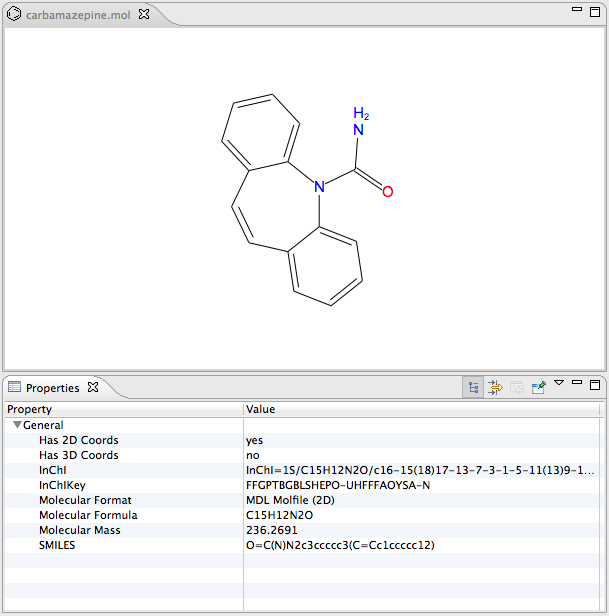
\includegraphics[width=9cm]{carbamazepine-props.png}

\caption{Part of the Bioclipse workbench showing the chemical structure for the drug carbamazepine, with the InChI and InChIKey displayed as properties in the bottom canvas. Editing the chemical structure instantly triggers a recalculation of these properties.}
\label{fig:carba-prop}
\end{center}
\end{figure*}


%InChI in Bioclipse
\subsection*{Integration of InChI in Bioclipse}
Bioclipse is a workbench for the life sciences where cheminformatics is the most developed functionality. Key features of Bioclipse includes import, export and editing of chemical structures in various file formats, as well as visualizations and various property calculations - all features available from both a graphical workbench as well as a built-in scripting language (Bioclipse Scripting Language, or BSL)~\cite{Spjuth:2009ly}. As a Rich Client built on the Eclipse Rich Client Platform (RCP), Bioclipse inherits an extensible architecture implementing the OSGi standard. By adding the previously described InChI OSGi bundles to Bioclipse, Bioclipse exposes InChI calculation as a key feature in the workbench, and InChI is calculated on all structure modifications and visualized as a general property in the workbench window (see Figure~\ref{fig:carba-prop}). Bioclipse supports both the generation of standard and non-standard InChIs, and a preference allows for selecting between the different versions.



\begin{verbatim}
  mol=cdk.fromSMILES("OC=O")
  sinchi = inchi.generate(mol);
  inchi = inchi.generate(mol), "FixedH");
\end{verbatim}


\begin{figure*}[!hb]
\begin{center}
	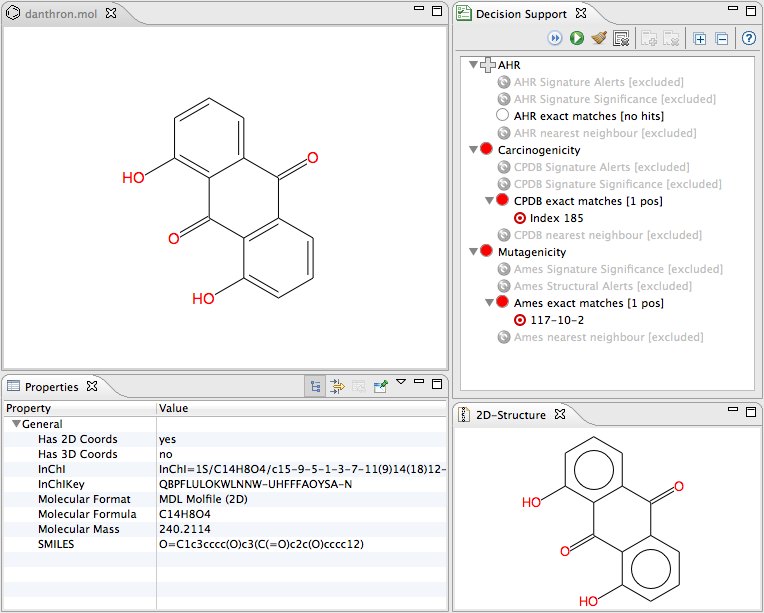
\includegraphics[width=9cm]{danthron-ds.png}

\caption{Part of the Bioclipse workbench showing the Decision Support feature with three exact matches enabled (right canvas) and the chemical structure of the withdrawn drug Danthron. We see that the data sets for CPDB~\cite{Fitzpatrick:2008dp} and Ames Mutagenicity~\cite{Kazius:2005pv} both gives an exact match, and that this compound has previously been shown to be positive (mutagen) in an Ames Mutagenicity test as well as positive for an in vivo carcinogenicity test included in the Carcinogenicity Potency Database.}
\label{fig:danth-ds}
\end{center}
\end{figure*}

	



%%%%%%%%%%
%APPLICATIONS
%%%%%%%%%%
\subsection*{Applications of InChI in cheminformatics}



\subsubsection*{a) Decision support in computational pharmacology}
In chemical safety assessment, the first step when faced with a new chemical structure is to see weather it already has been synthesized, and if any in vitro assays or in vivo studies have been performed. Given the large size of knowledge bases in companies and organizations, exact database lookups have become ubiquitous tools and used on a daily basis. Bioclipse Decision Support provides a framework for running exact match queries against a library of chemical structures, which was demonstrated for 3 open safety endpoints~\cite{Spjuth:2011qf}. An example query can be seen in Figure~\ref{fig:danth-ds}.


\subsubsection*{b) Linked data spidering in Bioclipse with Isbjørn}

Molecular structures on the internet can be searched using InChI and InChIKeys~\cite{Coles2005} directly.
However, they can also be used as seed to spider (the process of following links on the world wide web)
the Linked Data section of the World Wide Web~\cite{Samwald2011}. We developed a plugin to Bioclipse
that searches the Internet for information about a molecule, initiated with the InChI and a web service
we developed earlier, providing Universal Resource Identifiers for molecules, available
at \url{http://rdf.openmolecules.net/}~\cite{Willighagen2011}. This
service provides a number of initial links to other Linked Data resources, and links to other
resources are followed using owl:sameAs and skos:exactMatch predicates.

While spidering the web of molecular information, common ontologies are recognized and use to extract
information about the compound. Recognized ontologies include general ontologies like
Dublin Core (\url{http://dublincore.org/}), RDF Schema~\cite{Guha:04:RVD}, SKOS~\cite{Bechhofer:09:SSK},
and FOAF~\cite{Grav07}, as well as domain specific ontologies, like
ChemAxiom~\cite{Adams2009}, CHEMINF~\cite{Hastings2011}, and specific predicates
used by specific databases, including Bio2RDF~\cite{Belleau2008}, DBPedia~\cite{DBPEDIA},
and ChemSpider~\cite{Pence2010} (see Figure~\ref{fig:isbjorn} left).

But by educating Isbjørn about further ontologies we can even, for example, extract drug side effects
from the SIDER database~\cite{Kuhn2010}, as exposed by the Free University Berlin RDF services,
as shown in Figure~\ref{fig:isbjorn} right. The search results of Isbjørn are presented in Bioclipse
as a HTML page and opened in a browser window (not shown).

\begin{figure*}[!hb]
\begin{center}
	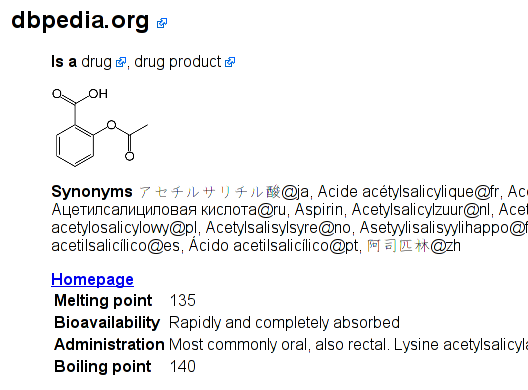
\includegraphics[width=7cm]{isbjorn6.png}
	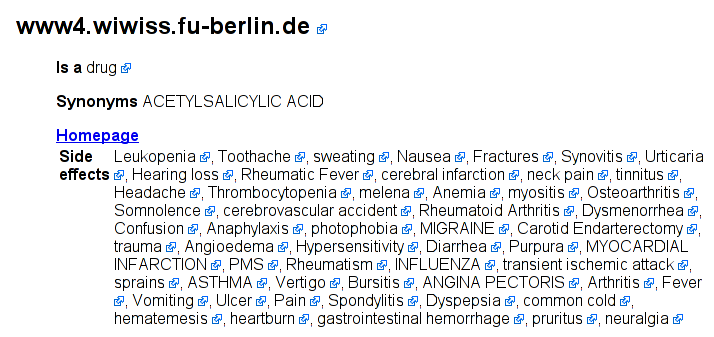
\includegraphics[width=7cm]{isbjorn8.png}
\caption{Screenshot of Linked Data spidering results by Isbjørn presented as a HTML page.}
\label{fig:isbjorn}
\end{center}
\end{figure*}


\subsubsection*{c) CDK tautomer calculation in Bioclipse moltable}

The InChI library can also be used to generate tautomers\cite{Thalheim2010}. This method has been
implemented in the CDK by Rijnbeek~\cite{Rijnbeek2011}, and exposed in the Bioclipse Scripting Language.
Tautomers can be calculated for any molecule, for example, created from a SMILES string in this
example for phenol:

\begin{verbatim}
// no aromatic rings that make it hard to
// see where the double bonds are
jcpglobal.setShowAromaticity(false);

inputSMILES = "c1ccccc1O";
inputName = "phenol";
inchi.generate(
  cdk.fromSMILES(inputSMILES)
)
tautomers = cdk.getTautomers(
  cdk.fromSMILES(inputSMILES)
)

file = "/Virtual/" + inputName + ".sdf";
cdk.saveSDFile(file, tautomers);
ui.open(file);
\end{verbatim}

Using this approach we can generate tautomers for any molecules, though it is limited by
the heuristic rules implemented by the InChI library. We typically only find a subset
of tautomers, rather than a full set. For example, for warfarin it finds only six tautomers
out of the 40 reported ones~\cite{Porter2010}.

%%%%%%%%%%%%%%%%%%%%%%
\section*{Conclusions}
The InChI project has chosen the path to rely on a single implementation for standardizing InChI calculations,
and it is important that this code is readily available for all cheminformatics software development. This paper
describes the packaging of InChI as a Java library using a JNI bridge (JNI-InChI), which is available as a Java
Archive (jar file), and as Maven bundles. It further shows the integration into the CDK library and
how the JNI-InChI as OSGi bundles renders InChI easily available for software using this dynamic module system,
such as the Bioclipse workbench. The various binary packages make the InChI library easily useable in
a variety of Java environments.

%Problems with InChI versions
A feature of the InChI is that it supports various layers of detail in describing the chemical structure,
which has confused end users of cheminformatics software. This resulted in a set of chosen layers, resulting
in the standard InChI. The CDK supports generation and processing of both the standard and non-standard InChIs.
Bioclipse provides a preference page where users can indicate which InChI they like to be calculated by
default.

%Implications
The uses in the CDK and Bioclipse have shown that the InChI is of great utility for uniquely identifying
molecular structures in a canonical form, and is therefore well suited for exact matches in database searches, 
as exemplified in computational pharmacology example. This makes it also highly suitable for mining the
internet and the Linked Data network. We demonstrate this with our Isbjørn plugin for Bioclipse, which
aggregates knowledge about chemical compounds from an increasing list of disparate sources. The use of the
InChI here shows the potential for the common task to collect as much information as possible about a
novel chemical structure, uniquely identified by the InChI. But the use of the InChI algorithms is not limited to
that purpose, and has further benefits. We demonstrate this with the exposure in the CDK and Bioclipse to
generate tautomers. 

% Limitations
Our results show that it is possible to overcome the problem that the InChI algorithm is not implemented
in Java, but this however comes at a price. Using non-Java code in a Java environment requires a bridge, for which
we used JNI, but crossing this bridge is computationally expensive. Furthermore, the integration into the
CDK requires bridging two data models: one for the CDK and one for the InChI library. A suite of unit
tests is in place to validate that information is correctly translated from the CDK data model into
calculted InChIs. However, a full validation using the InChI project test suite has not been completed
yet.

%%%%%%%%%%%%%%%%%%
%\section*{Methods}
%  \subsection*{Methods sub-heading for this section}
%    Text for this sub-section \ldots


    
%%%%%%%%%%%%%%%%%%%%%%%%%%%%%%%%
\section*{Authors contributions}
OS and EW wrote major parts of the manuscript and organized the paper writing process. SA wrote the JNI-InChI library and
the CDK integration. AB created the OSGi bundles. EW wrote Isbjørn plugin and application. OS, AB, and EW made the InChI
functionality available in Bioclipse. The decision support use case was developed by OS.
All authors read and approved the final manuscript.
    

%%%%%%%%%%%%%%%%%%%%%%%%%%%
\section*{Acknowledgements}
We acknowledge Mark Rijnbeek for implementing the InChI-based tautomer
generation in the CDK.

 
%%%%%%%%%%%%%%%%%%%%%%%%%%%%%%%%%%%%%%%%%%%%%%%%%%%%%%%%%%%%%
%%                  The Bibliography                       %%
%%                                                         %%              
%%  Bmc_article.bst  will be used to                       %%
%%  create a .BBL file for submission, which includes      %%
%%  XML structured for BMC.                                %%
%%                                                         %%
%%                                                         %%
%%  Note that the displayed Bibliography will not          %% 
%%  necessarily be rendered by Latex exactly as specified  %%
%%  in the online Instructions for Authors.                %% 
%%                                                         %%
%%%%%%%%%%%%%%%%%%%%%%%%%%%%%%%%%%%%%%%%%%%%%%%%%%%%%%%%%%%%%


{\ifthenelse{\boolean{publ}}{\footnotesize}{\small}
 \bibliographystyle{bmc_article}  % Style BST file
  \bibliography{inchi-cdk-bioclipse} }     % Bibliography file (usually '*.bib' ) 

%%%%%%%%%%%

\ifthenelse{\boolean{publ}}{\end{multicols}}{}

%%%%%%%%%%%%%%%%%%%%%%%%%%%%%%%%%%%
%%                               %%
%% Figures                       %%
%%                               %%
%% NB: this is for captions and  %%
%% Titles. All graphics must be  %%
%% submitted separately and NOT  %%
%% included in the Tex document  %%
%%                               %%
%%%%%%%%%%%%%%%%%%%%%%%%%%%%%%%%%%%

%%
%% Do not use \listoffigures as most will included as separate files

%\section*{Figures}
%  \subsection*{Figure 1 - Sample figure title}
%      A short description of the figure content
%      should go here.
%
%  \subsection*{Figure 2 - Sample figure title}
%      Figure legend text.



%%%%%%%%%%%%%%%%%%%%%%%%%%%%%%%%%%%
%%                               %%
%% Tables                        %%
%%                               %%
%%%%%%%%%%%%%%%%%%%%%%%%%%%%%%%%%%%

%% Use of \listoftables is discouraged.
%%
\section*{Tables}
  \subsection*{Table 1 - Various Java methods from the JniInChIWrapper class.}
  \label{tab:wrapper}
\begin{tabular}{ll}
\textbf{JniInChIWrapper} & \\
\hline
loadLibrary() & Loads the InChI library suitable for the platform. \\
getInchi(JniInchiInput) & Generates an InChI for the given input structure, with the \\
                        & InChI options passed with the input. \\
getStdInchi(JniInchiInput) & Generates a Standard InChI for the given input structure. \\
getStructureFromInchi(JniInchiInputInchi) & Generates a structure from an InChI string (without coordinates). \\
getInchiKey(String) & Converts an InChI into an InChIKey. \\
checkInchi(String, boolean) & Check the validity of a (non-standard) InChI either loosely or strict. \\
checkInchiKey(String, boolean) & Check the validity of a (non-standard) InChIKey either loosely or strict. \\
\hline
\textbf{JniInchiInput} & \\
\hline
JniInchiInput(List) & Constructor allowing you to set the InChI generation options \\
                     & as a List of Strings. \\
addAtom(JniInchiAtom) & Adds an atom to the input structure. \\
addBond(JniInchiBond( & Adds a bond to the input structure. \\
addStereo0D(JniInchiStereo0D) & Adds a tetrahedral, bond, or allene stereochemistry \\
                              & element to the input structure. \\
\end{tabular}

%    Here is an example of a \emph{small} table in \LaTeX\ using  
%    \verb|\tabular{...}|. This is where the description of the table 
%    should go. \par \mbox{}
%    \par
%    \mbox{
%      \begin{tabular}{|c|c|c|}
%        \hline \multicolumn{3}{|c|}{My Table}\\ \hline
%        A1 & B2  & C3 \\ \hline
%        A2 & ... & .. \\ \hline
%        A3 & ..  & .  \\ \hline
%      \end{tabular}
%      }
%  \subsection*{Table 2 - Sample table title}
%    Large tables are attached as separate files but should
%    still be described here.



%%%%%%%%%%%%%%%%%%%%%%%%%%%%%%%%%%%
%%                               %%
%% Additional Files              %%
%%                               %%
%%%%%%%%%%%%%%%%%%%%%%%%%%%%%%%%%%%

%\section*{Additional Files}
%  \subsection*{Additional file 1 --- Sample additional file title}
%    Additional file descriptions text (including details of how to
%    view the file, if it is in a non-standard format or the file extension).  This might
%    refer to a multi-page table or a figure.
%
%  \subsection*{Additional file 2 --- Sample additional file title}
%    Additional file descriptions text.


\end{bmcformat}
\end{document}







